\section{Unity}
\subsection{Sučelje}
Glavno sučelje unity-a sadrži više prozora koji se mogu grupirati po želji korisnika. Sučelje se sastoji od alatne trake. hierarhijskog prozora, pogleda na scenu, inspektora i prozora projekta.

\subsubsection{Prozor projekta}
Prozor projekta prikazuje sve datoteke koje se koriste u projektu. Preporučava se napraviti direktorije u kojima se raspoređuju skripte, zvukovi, animacije i ostali objekti. Kada uključujemo neke segmente u projekt oni će se pojaviti u prozoru projekta.


\subsubsection{Alatna traka}
Alatna traka omogućuje najbitnije funkcionalnosti za kreiranje igre. Na lijevoj strani se nalaze alati pomoću kojih možemo upravljati sa scenom i sa objektima koji su u sceni. Objektima možemo postaviti visinu, dužinu, koordinate trenutnog položaja itd. Na sredini se nalaze "play", "pause" i "stop" kontrole koje omogućuju testiranje igre. Na desnoj strani se nalaze kontrole za oblak servis i osobni unity račun te kontrole za postavljanje rasporeda sučelja po korisnikovoj želji.

\subsubsection{Pogled na scenu}
Scena nam prikazuje 3D ili 2D objekte, ovisno o vrsti projekta na kojem radimo. Pogled na scenu omogućava programeru da vizualno upravlja svojom igrom. Osim pogleda na scenu imamo i pogled na igru (game view) koji programeru omogućva testiranje svoje igre te pronalaženje pogrešaka.


\subsubsection{Hierarhiski prozor}
Ovdje možemo vidjeti kako su objekti pridruženi drugim objektima vizualno, što pomaže pri pisanju koda. Hierarhiski prozor će prikazati one objekte koji su u sceni koju trenutno uređujemo.

\subsubsection{Konzola}
Konzola nas obavještava kada se dogodi neka greška, upozorenje ili iznimka. Konzola je dosta praktična jer  preko nje možemo saznati što nam se u kojem trenutku događa u projektu i to preko funkcije "Debug.Log()". 

\subsubsection{Inspektor}
Inspektor omogućuje da imamo uvid u sva svojstva trenutno odabranog objekta. Preko njega možemo mjenjati komponente objekta. Odabirom nekog objekta inspektor ce automatski komponente tog objekta prikazati u svom prozoru.




\begin{center}
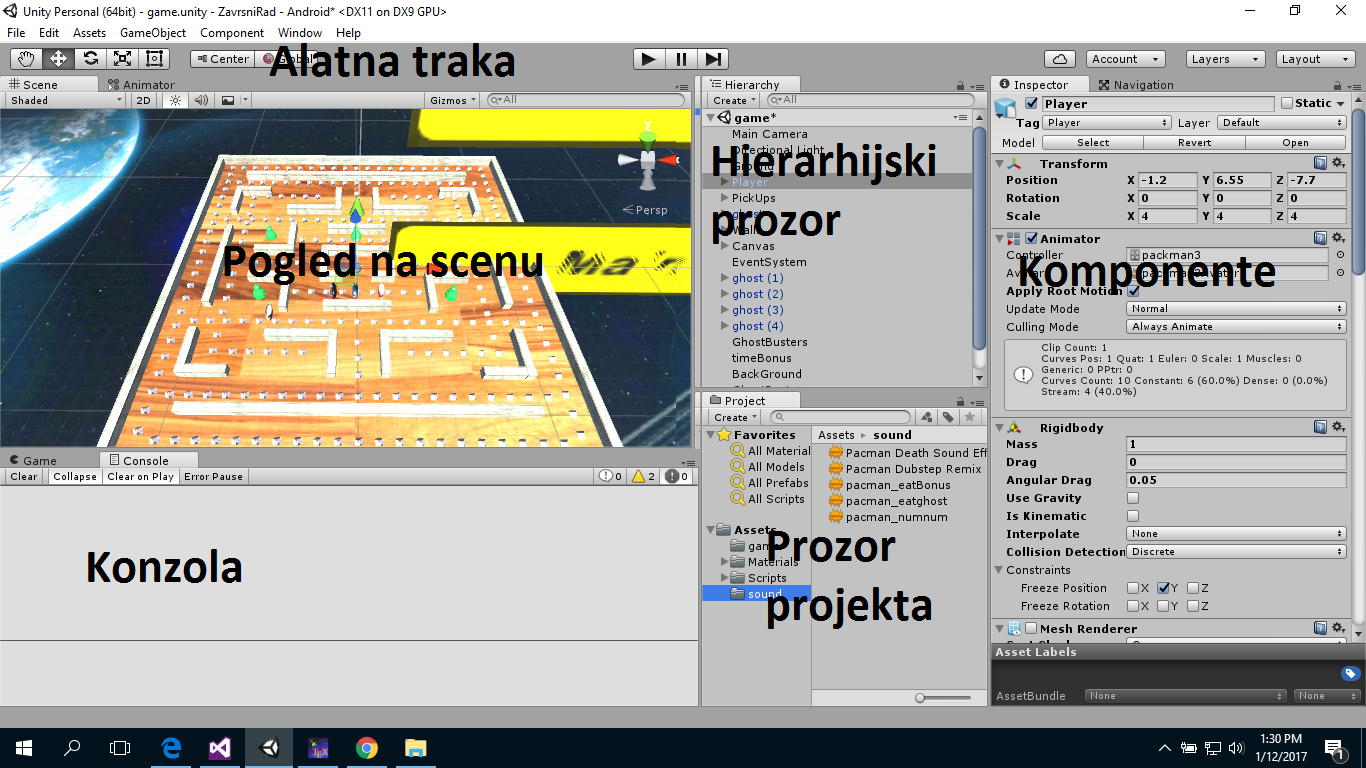
\includegraphics[scale=0.35]{interface.png}

Slika 1: Prikaz sučelja
\end{center}

\subsection{Assets}
Assets-i su ukjučeni ili kreirani objekti. Assets-i mogu biti 3D modeli, zvuk, tekst itd. Kada neki objekt uključimo u unity on će se automatski pojaviti u asset direktoriju.


\subsection{Objekti}
Sve što se nalazi na sceni je objekt. Objekti se mogu kreirati u unity-u ili pridružiti ih iz drugog alata. Svaki objekt u sebi sadrži sljedeće osobine: ime, tag, sloj i static. Autor sam može proizvoljno dati ime svom objektu po želji. Tagovi su jako poželjni kada se referenciraju objekti u kodu. Traženje objekata preko tagova olakšava posao programeru pogotovo kada se radi na većim projektima. Kada više razlićitih objekata rade istu stvar onda je poželjno koristiti tag. Objekti mogu biti dodjeljeni drugom sloju. Static se koristi za objekte koji su statični.


\subsection{Komponente}
Svaki objekt mora sadržavati neke komponente. Pri kreiranju objekta njemu će se dodjeliti "Transform" komponenta koja prikazuje poziciju, rotaciju i visinu objekta. Bez ove komponente objekt bi bio nevidljiv na sceni. Neke od komponenata su "Character Controller", "Nav Mesh Agent", "Rigidbody" itd.


\subsection{Montaža (Prefab)}
Prefab možemo gledati kao objekt na koji je korisnik postavio instancu. Kada se napravi neka promjena na prefabu ta promjena će se primjeniti za instance tog objekta.

\subsection{Pisanje koda}
\subsubsection{Programski jezici}
U unity platformi se može kreirati igra korištenjem jednog od tri programska jezika,a oni su c sharp, javaScript i Boo. Prednosti c sharp programskog jezika prema java scriptu je to što se lakše otkrivaju pogreške u kodu. Java script se često koristi u Unity-u. Često se naziva i Unity Script. Prednosti java scripta prema c sharp-u su jednostavnija sintaksa java script programskog jezika i mnogo primjera koje se mogu naći na internetu. Programski jezik Boo se jako malo koristi u Unity-u i ima samo nekolicinu primjera na internetu što korisnika automatski udaljuje od ovog jezika. 


\subsubsection{Petlje}
Kada se kreira skripta unity će automatski kreirati "Start()" funkciju i "Update()" petlju. "Awake()" funkcija je funkcija koja će se prva pozvati kada se igra pokrene i ona se poziva samo jednom. "Awake()" funkcija se najčešće koristi da se u nju postave reference između skripti jer se objekti još nisu izvršili. "Start()" funkcija će se pozvati nakon "Awake()" funkcije, ona se poziva kada se svi objekti iz scene izvrše. "Start()" funkcija će se također pozvati samo jednom. "Start()" funkcija je najbolje mjesto za postaviti refence objekata. Nakon funkcije "Start()" unity ce pozvati petlju "Update()". Postoje dvije takve petlje a to su "Update()" i "Fixedupdate()". Petlja se izvršava onoliko puta po sekundi koliko je računalo može procesuirati. Razlika između ove dvije petlje je ta što se "FixedUpdate()" izvršava u određenom vremenu.
\begin{center}
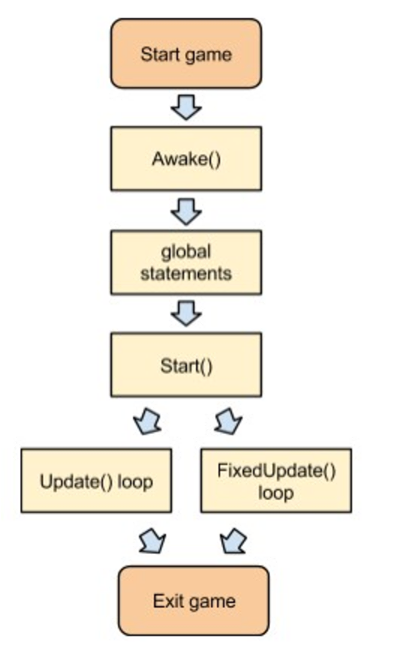
\includegraphics[scale=0.65]{loop.png}


Slika 2: Arhitektura igre
\end{center}
\subsection{Fizika}
Svaki objekt koji ima veze sa fizikom mora sadržavati RigidBody i Collider komponente. Glavne komponente RigidBody-a su "Use Gravity" i "Is Kinematic".
"Use Gravity" jednostavno znači da će se tom objektu postaviti gravitacija s obzirom na komponentu "Mass". Komponenta "Is Kinematic" se koristi kada korisnik želi tokom igre upravljati sa objektom preko transfom funkcije. "Use Gravity" i "Is Kinematic" komponente su tipa bool i njih postavljamo u inspektoru.

\subsection{Kamera}
Svaka scena mora sadržavati barem jednu kameru. Kada se scena kreira kreira se i objekt glavna kamera. Preko kamere određujemo da li je igra "first person game" ili "third person game".







